%%
%% This is file `sample-sigconf.tex',
%% generated with the docstrip utility.
%%
%% The original source files were:
%%
%% samples.dtx  (with options: `sigconf')
%% 
%% IMPORTANT NOTICE:
%% 
%% For the copyright see the source file.
%% 
%% Any modified versions of this file must be renamed
%% with new filenames distinct from sample-sigconf.tex.
%% 
%% For distribution of the original source see the terms
%% for copying and modification in the file samples.dtx.
%% 
%% This generated file may be distributed as long as the
%% original source files, as listed above, are part of the
%% same distribution. (The sources need not necessarily be
%% in the same archive or directory.)
%%
%% The first command in your LaTeX source must be the \documentclass command.
\documentclass[sigconf]{acmart}
%%%% As of March 2017, [siggraph] is no longer used. Please use sigconf (above) for SIGGRAPH conferences.

%%%% Proceedings format for SIGPLAN conferences 
% \documentclass[sigplan, anonymous, review]{acmart}

%%%% Proceedings format for SIGCHI conferences
% \documentclass[sigchi, review]{acmart}

%%%% To use the SIGCHI extended abstract template, please visit
% https://www.overleaf.com/read/zzzfqvkmrfzn

%%
%% \BibTeX command to typeset BibTeX logo in the docs
\AtBeginDocument{%
  \providecommand\BibTeX{{%
    \normalfont B\kern-0.5em{\scshape i\kern-0.25em b}\kern-0.8em\TeX}}}


%%
%% Submission ID.
%% Use this when submitting an article to a sponsored event. You'll
%% receive a unique submission ID from the organizers
%% of the event, and this ID should be used as the parameter to this command.
%%\acmSubmissionID{123-A56-BU3}

%%
%% The majority of ACM publications use numbered citations and
%% references.  The command \citestyle{authoryear} switches to the
%% "author year" style.
%%
%% If you are preparing content for an event
%% sponsored by ACM SIGGRAPH, you must use the "author year" style of
%% citations and references.
%% Uncommenting
%% the next command will enable that style.
%%\citestyle{acmauthoryear}

%%
%% end of the preamble, start of the body of the document source.
\begin{document}

%%
%% The "title" command has an optional parameter,
%% allowing the author to define a "short title" to be used in page headers.
\title{Computer Vision Runescape Botting with YOLOv3 and Adversarial Methods}

%%
%% The "author" command and its associated commands are used to define
%% the authors and their affiliations.
%% Of note is the shared affiliation of the first two authors, and the
%% "authornote" and "authornotemark" commands
%% used to denote shared contribution to the research.
\author{Patrick Kidd}
\email{pnk5@rice.edu}
\affiliation{%
  \institution{Rice University}
  \streetaddress{6350 Main St}
  \city{Houston}
  \state{Texas}
  \postcode{77005}
}

%%
%% By default, the full list of authors will be used in the page
%% headers. Often, this list is too long, and will overlap
%% other information printed in the page headers. This command allows
%% the author to define a more concise list
%% of authors' names for this purpose.
\renewcommand{\shortauthors}{Patrick Kidd}

%%
%% The abstract is a short summary of the work to be presented in the
%% article.
\begin{abstract}
  I develop a neural network for computer vision based on the YOLOv3-Tiny architecture and train it to detect iron ore in Runescape. The neural network is run on direct screen output in conjunction with some user input heuristics to autonomously play Runescape in a human-like manner with no visibility of game data or other objects in memory.
\end{abstract}

\ccsdesc[100]{Networks}
\ccsdesc[100]{Computer Vision}
\ccsdesc[100]{CNNs}

%%
%% Keywords. The author(s) should pick words that accurately describe
%% the work being presented. Separate the keywords with commas.
\keywords{neural networks, computer vision, spoofing, YOLOv3}

%% A "teaser" image appears between the author and affiliation
%% information and the body of the document, and typically spans the
%% page.
\begin{teaserfigure}
  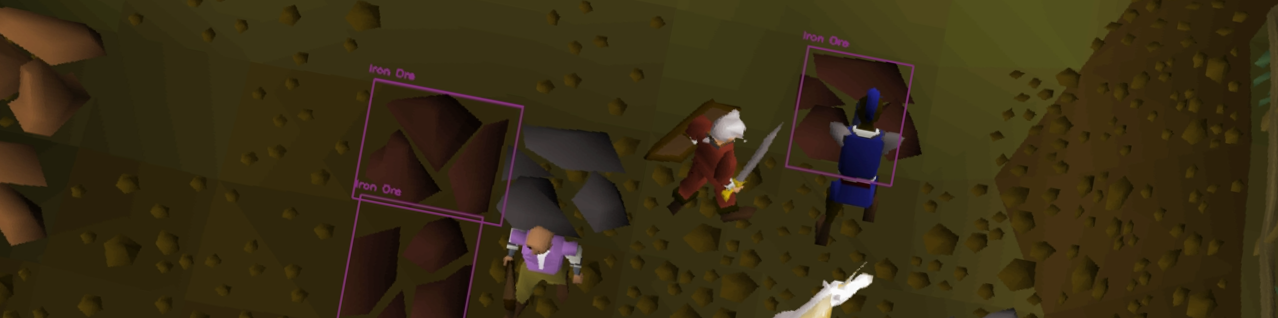
\includegraphics[width=\textwidth]{newtop.png}
  \caption{The Bot at Work, 2019.}
  \Description{Computer vision boundaries drawn in.}
  \label{fig:teaser}
\end{teaserfigure}

%%
%% This command processes the author and affiliation and title
%% information and builds the first part of the formatted document.
\maketitle

\section{Introduction}
The use of computers as human-like interlocutors is an issue that was conceptualized at the latest by Alan Turing, and has been a pillar of networked system operation since at least 1992 when the Network Working Group published their survey of the field of network conferencing and noted the implications of botting on the resiliency of such systems. \cite{NWG01}

Throughout the 2000s, botting that began with IRC spread to video games, where profit could be made in leveling players' accounts, selling accounts, or manipulating competitive matches. These bots rely on game data to make decisions, which has become increasingly more difficult to access as developers have sought to choke off access to these unwanted programs. \cite{Cano01}

Acquiring game data for use in the bots has traditionally meant extracting state data from memory. As the opening chapter of Nick Cano's seminal work on game botting proclaims in the first paragraph, "Knowing a game's state is paramount to interacting with thte game intelligently, but unlike humans, software can't determine the state of a game simply by looking what's on the screen." \cite{Cano01} This has meant the battleground for game and bot developers has centered around memory access.

The primacy of memory has begotten ever more complex methods of process injection, driver bug exploitation, and even physical memory snooping for bot developers, met by increasingly complex tamper-detection, in-transit encryption, and self-monitoring processes for game developers.\cite{Cano01}

In the face of cheap, open-source, and (most crucially) fast computer vision, not only is all such work obsoleted, the concept of anti-botting itself may be rendered impossible. Computer vision, by scraping nothing more than the output visible to the human player itself interacts with the game in a way fundamentally indistinguishable from the human player. Even worse for game developers, many computer vision networks have been developed with the express aim of application to real-time detection of objects in the physical world. \cite{YOLO} This means that even should vendors find a way to secure screen output to intrusion all the way to the final output device, because humans must ultimately interpret the output via the patterns of light produced, the game is vulnerable to a raspberry pi with a webcam plugged in.

Having thus been forced to concede the question of input to bots, the only refuge for game developers will be policing of \textit{inputs to the game}, attempting to discern bots from legitimate players through their interaction with the game alone. This too may ultimately prove futile given the progress that has been made recently with OpenAI Five and Dota 2, where full teams of AI have consistently defeated the most skilled collections of professional players in their games. \cite{OpenAI}

Research conducted by Ontañón et. al in Starcraft 2 bots has discovered that many problems in real time strategy games originally deemed too difficult for bots, such as pathfinding, and low-scale micromanagement of units and production have been effectively solved.\cite{SC2} While the solution to most issues is though to belong with larger and more efficient CNN techniques however, several key components of gameplay remain unavailable to bots, among them adaptation to opponent strategy, learning from non-training or intra-game experience, and learning through outcomes of \textit{other players} in the same game. These constitute the final barrier to general bot feasibility across all games.\cite{SC2}

This paper will first discuss the implementation of YOLOv3 in interpreting screen output, and then more briefly touch on potential methods of adversarial machine learning to differentiate the resulting bot from genuine human input.

\section{Relevant Work}
\subsection{AlexNet: The Foundation}

Computer vision has been synonymous with convolutional neural networks since AlexNet completed the ImageNet Large Scale Visual Recognition Challenge in 2012. \cite{AlexNet} One of the most significant aspects of the AlexNet victory was its use of CUDA (The Nvidia non-graphical compute api) to accelerate both neural network training and execution with large GPU compute units. In the seven years since the release of AlexNet, transistor density of TSMC-fabricated Nvidia chips has more than doubled, making the already-cheap cost of Alex-style CNN all the more so.\cite{Nvidia10}

AlexNet's structure consists of 5 convolutional layers and 3 fully connected layers, operating on an initial 227x227x3 layer that is a random crop of a 256x256 image resulting from scaling performed on all input images.\cite{AlexNet} A diagram of the network architecture is visible in \textbf{figure 5} on the next page. From the input, AlexNet consists of interleaving convolutional and overlapping max-pool layers, terminating in two fully connected layers of 4096 neurons and a 1000-long softmax. \cite{UnderAlexNet}

AlexNet is also significant in having popularized the use of Rectified Linear Unit Nonlinearity (ReLU) to accelerate the training of neural networks. Where before Tanh and sigmoid functions were in widespread use, RelU is superior in allowing for positive output greater than one for positive z-values without distorting output on negative-z, resulting in faster convergence with gradient descent. \cite{UnderAlexNet}

There was one additional technique implemented in AlexNet that became central to many neural network designs, and is included in the YoloV3 architecture that is the foundation of the paper here, the idea of dropout. In AlexNet, each neuron has a 50\% probability of being dropped for an iteration, meaning that it does not contribute to forward \textit{or} back propagation, although the complete network is used for testing and ultimate production (with scaling of output to account for dropped neurons). While this naturally raises the number of iterations necessary for convergence and thus training, it greatly mitigates the risk of overfitting and is a more robust solution than random training image transforms. \cite{UnderAlexNet}

The resulting network holds 60 million parameters and 650,000 neurons, taking six days to train from scratch on the ImageNet Large Scale Visual Recognition Challenge using two GTX 580s.\cite{UnderAlexNet}

\subsection{You Only Look Once v3 (YOLOv3)}

\begin{figure}
  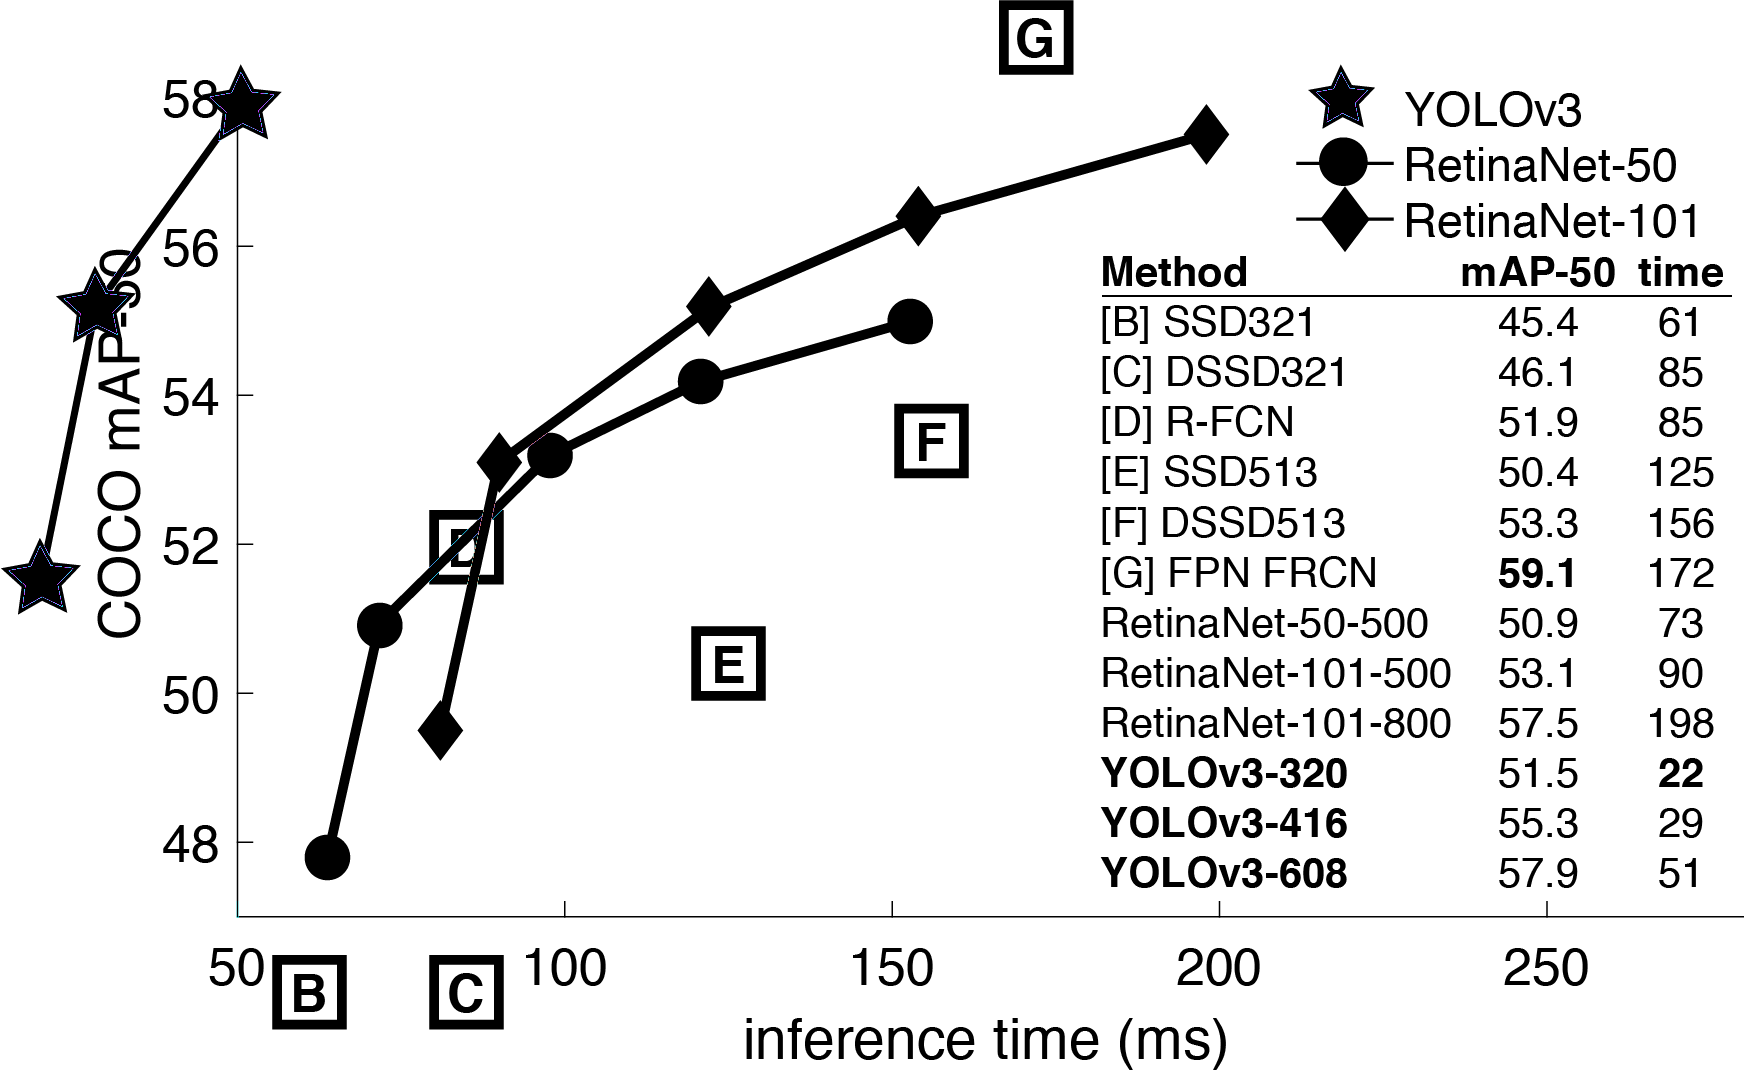
\includegraphics[width=0.45\textwidth]{map50blue.PNG}
  \caption{mAP of Selected Network Architectures}
  \label{fig:iterchart}
\end{figure}
\begin{figure}
  $\frac{True Positives}{True Positives + False Positives}$
  \caption{Precision}
  \label{fig:ap}
\end{figure}
\begin{figure}
  $\frac{True Positives}{True Positives + False Negatives}$
  \caption{Recall}
  \label{fig:rec}
\end{figure}
\begin{figure*}[h]
  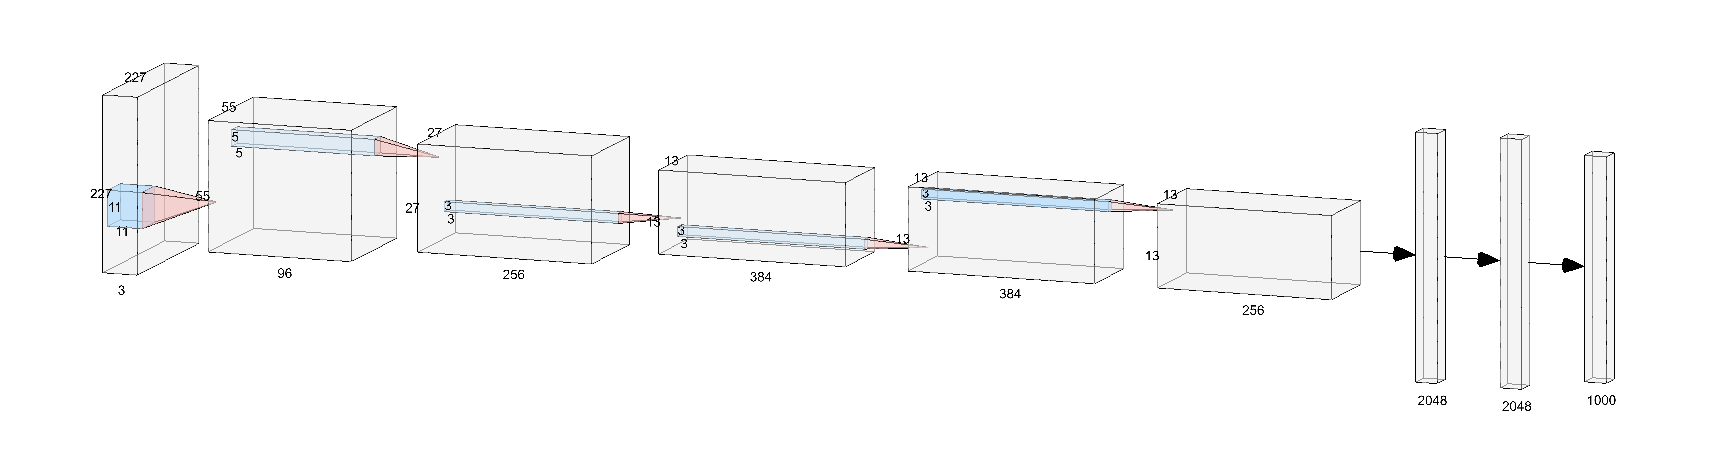
\includegraphics[width=\textwidth]{alexnetflat.PNG}
  \caption{AlexNet architecture.}
  \Description{Computer vision boundaries drawn in.}
  \label{fig:alex}
\end{figure*}

You Only Look Once v3 is the third iteration of a computer vision framework developed by Joseph Redmon and Ali Farhadi at the University of Washington. \cite{YOLO} Where other, extremely accurate champions of image-set tests have continued to focus on improvements in mAP and other measures of answer quality, YOLO was developed in the pursuit of speed. This speed is evident both in the number of iterations required to train a usable neural network, and in the speed of inference of that neural network in application. \cite{YOLO} \textbf{Figure 2} shows the performance of YOLOv3 relative to other, deeper, popular neural networks on the COCO training and test sets for a given inference time. mAP in this context is the area of the precision-recall curve obtained by the network where precision is the accuracy of the predictions themselves, defined as the ratio of true positives to the sum of true positives and false positives, and recall is the ratio of true positives to the sum of true positives and false negatives (\textbf{figures 3, 4}).

The ultimate output of YOLOv3 is four coordinates, representing a bounding box for each object detection $$b_x=\sigma(t_x)+c_x$$ $$b_y=\sigma(t_y)+x_y$$ $$b_w=p_we^{t_w}$$ $$b_h=p_he^{t_h}$$ where $c_x,x_y$ are absolute offsets in the image, and $p_w,p_h$ are prior width and height.

Training is done using logistic regression with sum of squared error loss where the gradient is computed as per-pixel truth minus the prediction. The logistic regression returns 1 for the bounding box that most overlaps the ground truth object in comparison to prior boxes, discarding boxes that are inferior but overlap beyond an arbitrary threshold (in the author's case 0.5). \cite{YOLO}

In the original author example, multilabel classification is used to enable classification of both parent and children classes, but as the implementation in this paper involves only a single class, such is not relevent to the application. \cite{YOLO}

One of the final crucial benefits of the prior work done by Messrs Redmon and Farhadi is the adaptability of their weight definitions to cut-down versions of their network. This means that any neural network which is a subset, either in layers or in components of layers, of the original YOLOv3 can begin training from weights pre-trained in the full model, thus allowing the end-user to tailor the accuracy-speed tradeoff to the optimum for their particular application.\cite{YOLO}

\subsection{Computer Vision in Games}

Prior to my work here, computer vision as a tool for gamestate data collection has not appeared in any paper to my knowledge, however several GitHub projects exists demonstrating the realtime game-interpretation capability of YOLOv3. \cite{Pine}

The most complete of these projects, Pine, does not however presently include botting, nor does the author intend to extend the purpose and capabilities of the network or script beyond aim-assistance in Counter-Strike: Global Offensive as visible in \textbf{figure 6}. \cite{Pine}

\begin{figure}
  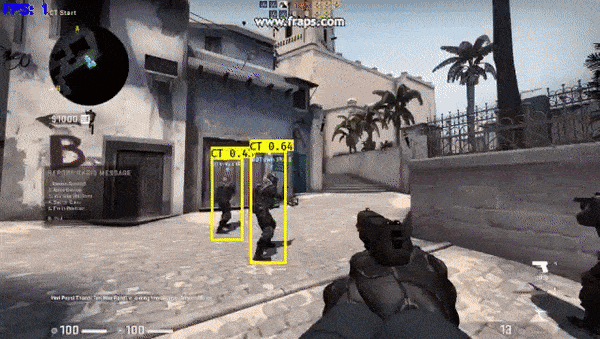
\includegraphics[width=0.45\textwidth]{csgo.png}
  \caption{Pine Aim Assistance in CS:GO}
  \label{fig:iterchart}
\end{figure}

\section{Methods}

\subsection{Data}

No appropriate dataset existed for this problem before my initiation of the project. Given, however, the ability of YOLOv3 to be trained on relatively small datasets, the creation of a purpose-collected labelled computer vision training set for Old School Runescape was not infeasible.

I captured 252 images of ore pits in Old School Runescape at my native resolution of 2560x1440, including the windows task bar that would be present in full screen captures from the wild. The images were stored as 8-bit PNGs without transparency.

Using labelImg I manually defined bounding boxes on all not-depleted iron ore visible in the images as in \textbf{figure 7}.\cite{Label} Resulting in Pascal VOC format per-image, per-box, per-class tagging that I converted to YOLOv3 tagging format in Python, which consists of a text file whose name matches every image name containing tab-delimited sets of classes and coordinates for each bounding box present in the image whose filename matches that of the text file.

The image set was selected to contain 25\% images with one ore, 25\% images with 2 ore, 25\% images with 3 ore, and 25\% images with 4 ore.

\begin{figure}
  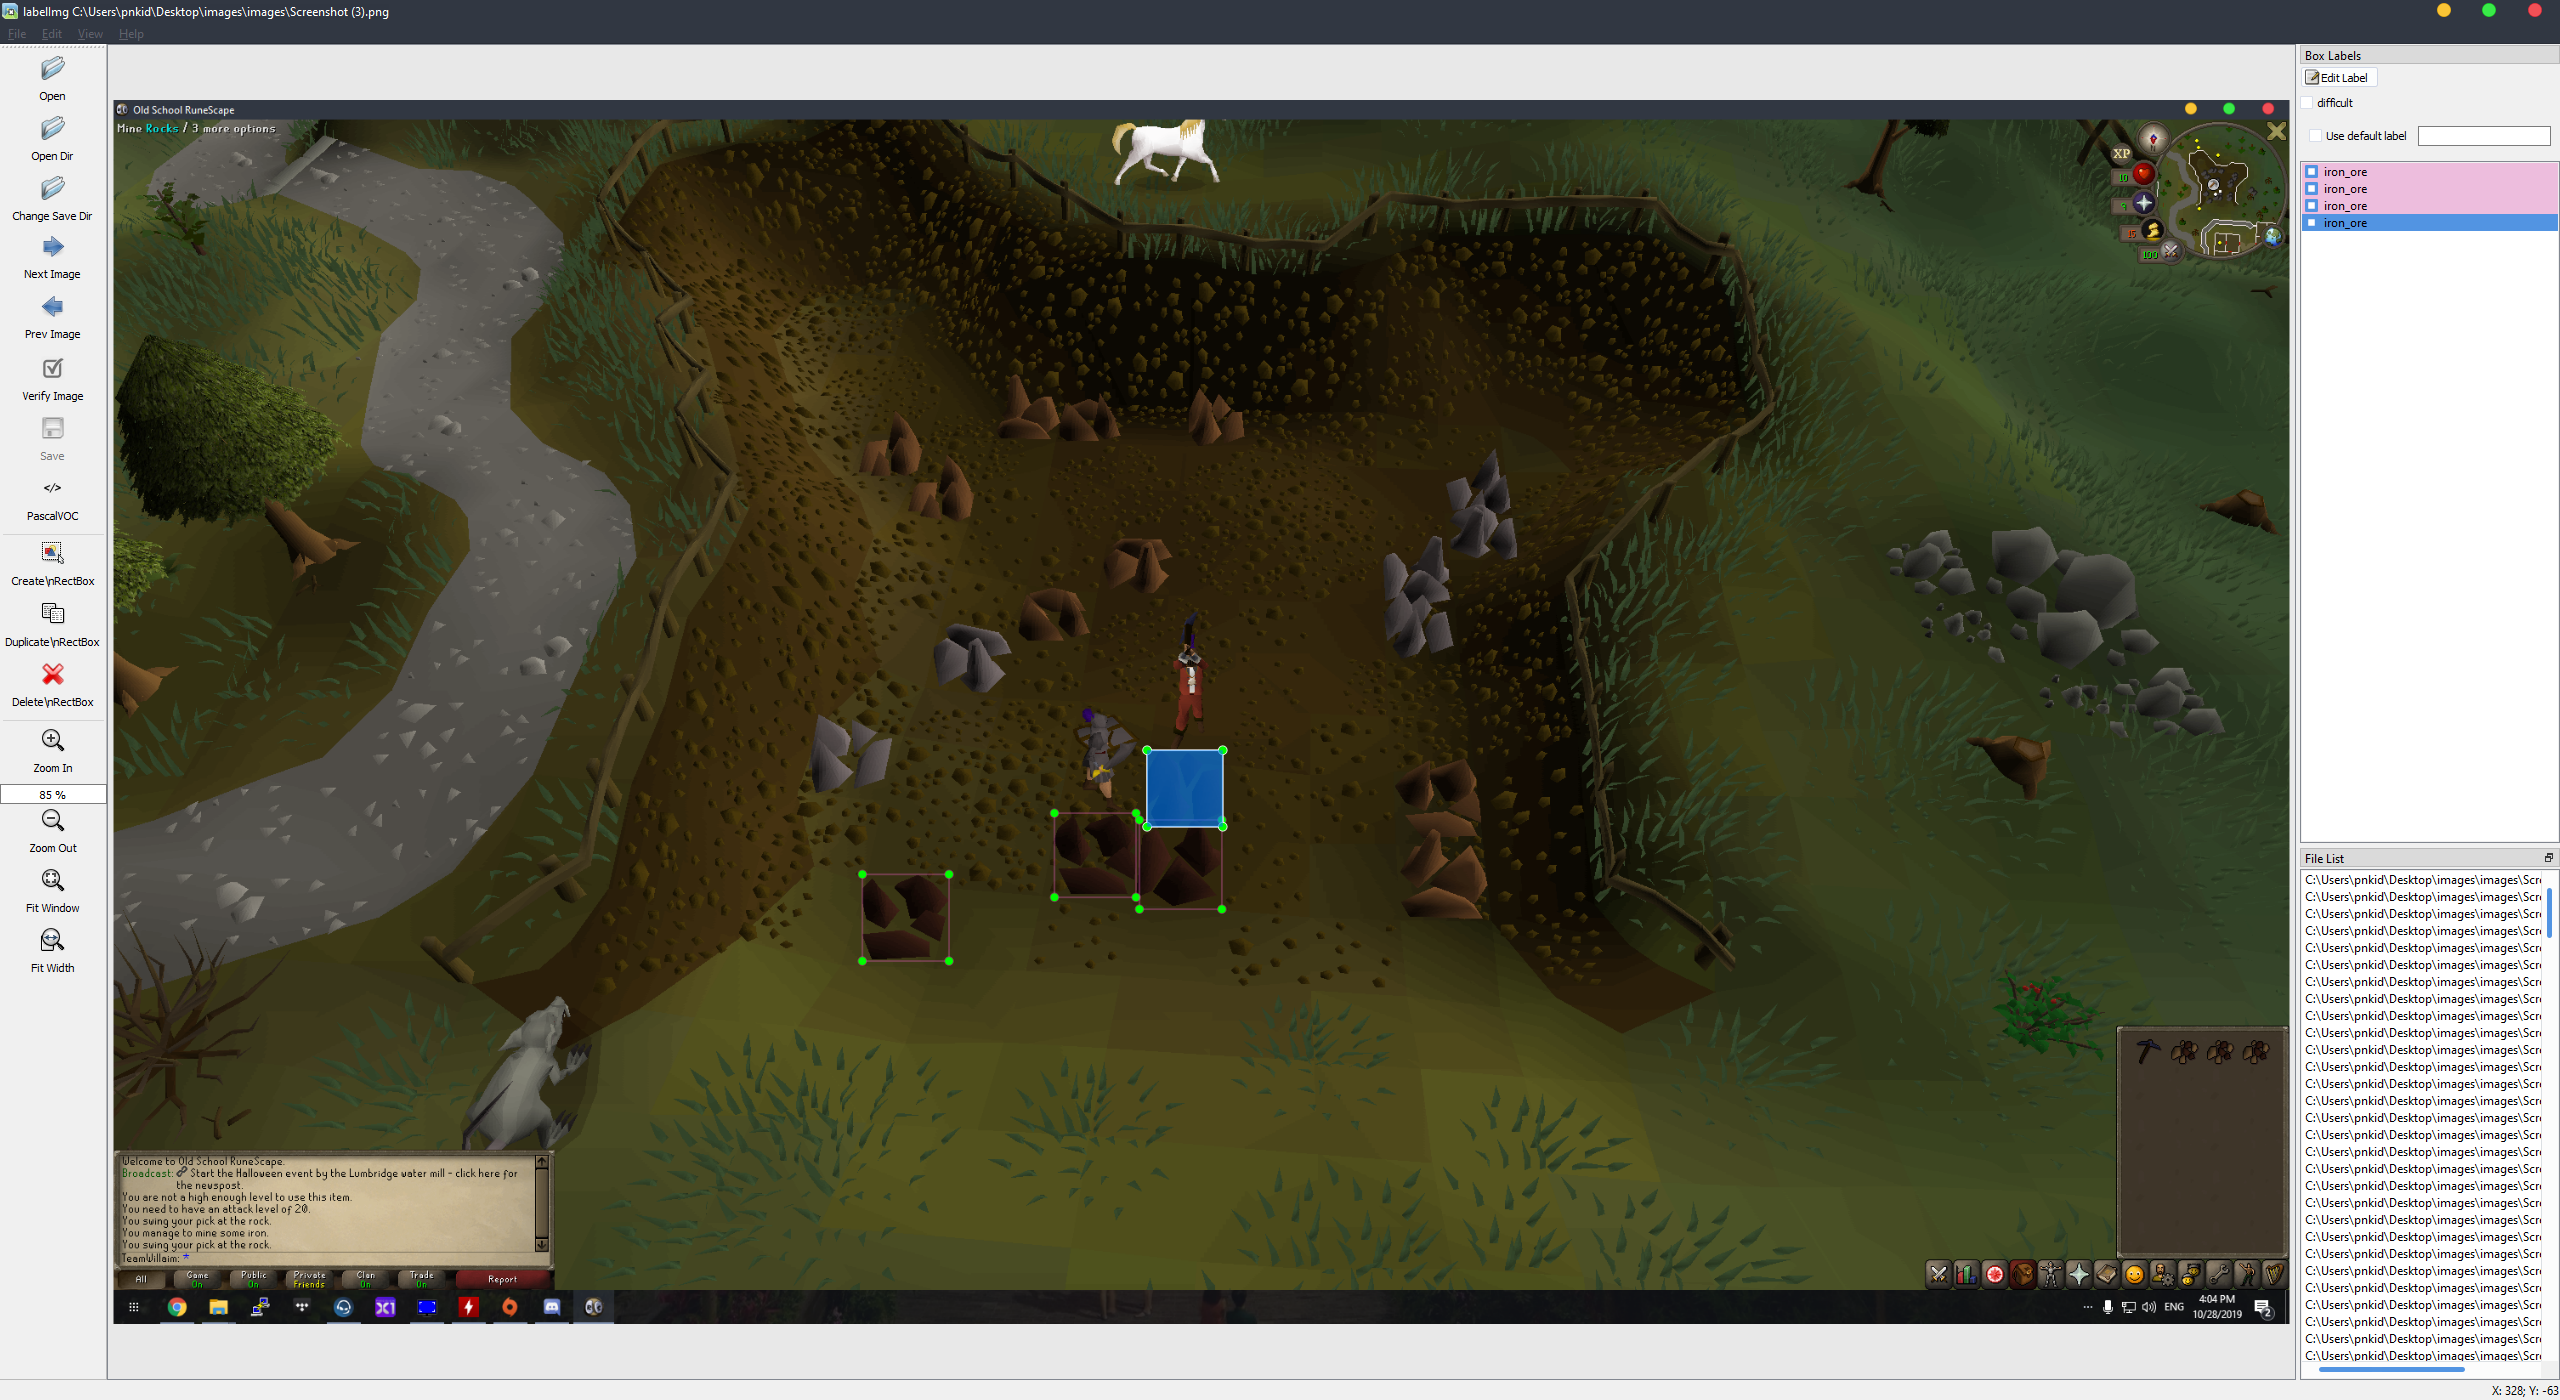
\includegraphics[width=0.45\textwidth]{labelled.png}
  \caption{Labelled Ore Images}
  \label{fig:iterchart}
\end{figure}

\subsection{Algorithms}
\subsubsection{YOLOv3 Tiny}

YOLOv3 Tiny is a network design that is essentially a subset of the original YOLOv3 network whose aim is even faster training and inference, and is able to leverage the large-model training weights as previously mentioned.

The architecture of YOLOv3 still operates on inputs scaled to RGB 416x416 images, and consists primarily of interleaved convolutional and max pooling layers, with the primary differences being a smaller number of layers overall, and most most consequentially pyramiding at \textit{2 levels} rather than 3. Pyramiding as used in YOLOv3 uses several upsampled layers at 3 different scales to help ensure consistent detection across the absolute scale of an object in the image, where YOLOv3 makes the sacrifice of sampling only at 13x13 and 26x26. The full design for YOLOv3 Tiny is defined in \textbf{figure 8}, with a graphical representation visible in AlexNet style in \textbf{figure 10} on the following page.

\begin{figure}[h]
  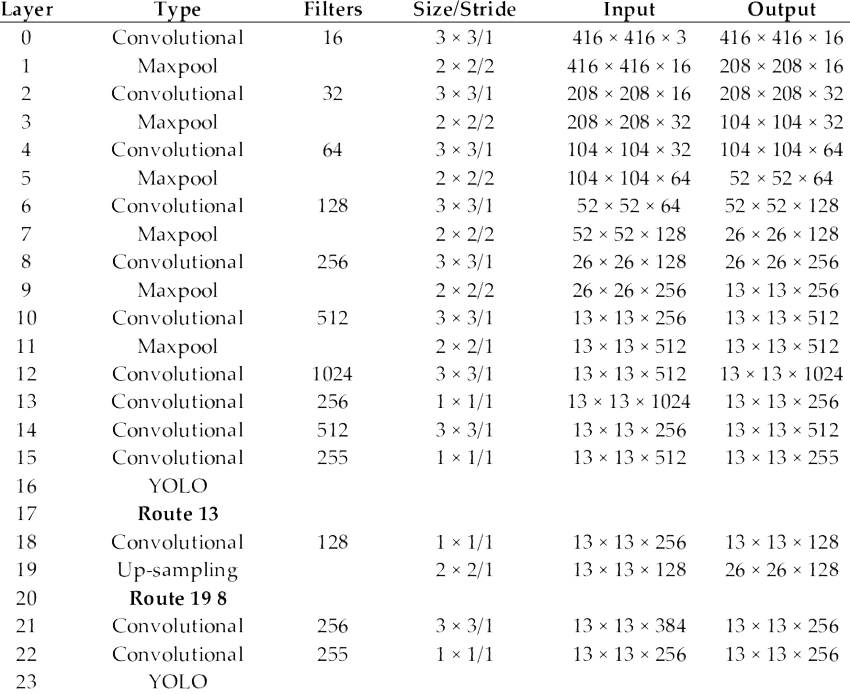
\includegraphics[width=0.45\textwidth]{table.PNG}
  \caption{YOLOv3 Tiny Architecture}
  \label{fig:tinytable}
\end{figure}

\subsubsection{OpenCV and Bot}

While Old School Runescape is not graphically demanding by modern standards, in order to make the bot framework more broadly applicable, I opted to use CPU-compiled OpenCV for inference. In most systems the performance bottleneck for players is their graphics processing, meaning pushing detection to the GPU will result in both sub-optimal inference performance \textit{and} degraded game responsiveness, both of which are undesirable for bot operation. \cite{GN}

Most video games are however poorly-threaded by virtue of a desire for console desirability, linear-progress requirements, and convention. This means that in an era where sub-\$200 consumer silicon is capable of high-IPC 6-core/12-thread performance, there is a considerable amount of under-utilized processing power resident in the CPU for most users while gaming. \cite{GN}

For expansion into other games therefore, it is desirable to operate the computationally-expensive inference loop on idle CPU cores rather than the much-faster GPU, hence my choice of OpenCV and python for detection and bot logic itself.


\section{Results}
\subsection{Network}

Unfortunately I had issues compiling Darknet with CUDA using Visual Studio and CMake, forcing me to use VCPKG. This may have had performance implications for the compiled binaries, and as such the performance may not be directly comparable (potential performance gains may be possible in such a low-threaded application through use of Intel C++ and G++ compilers with CUDA).\cite{Compile}

Nonetheless, training commenced from the weights obtained in the full YOLOv3 network that completed ImageNet, "darknet53.conv.74." In 18 hours of training on a single TU-104-400A die at an average clock of 2060mhz and average memory clock of 8225mhz across 8GB of GDDR6, more than 180,000 iterations were completed (with 180,000 the last saved checkpoint). Summary of the final network and the 5.448GFLOPS of computation can be seen in \textbf{Figure 10}.

\begin{figure*}[h]
  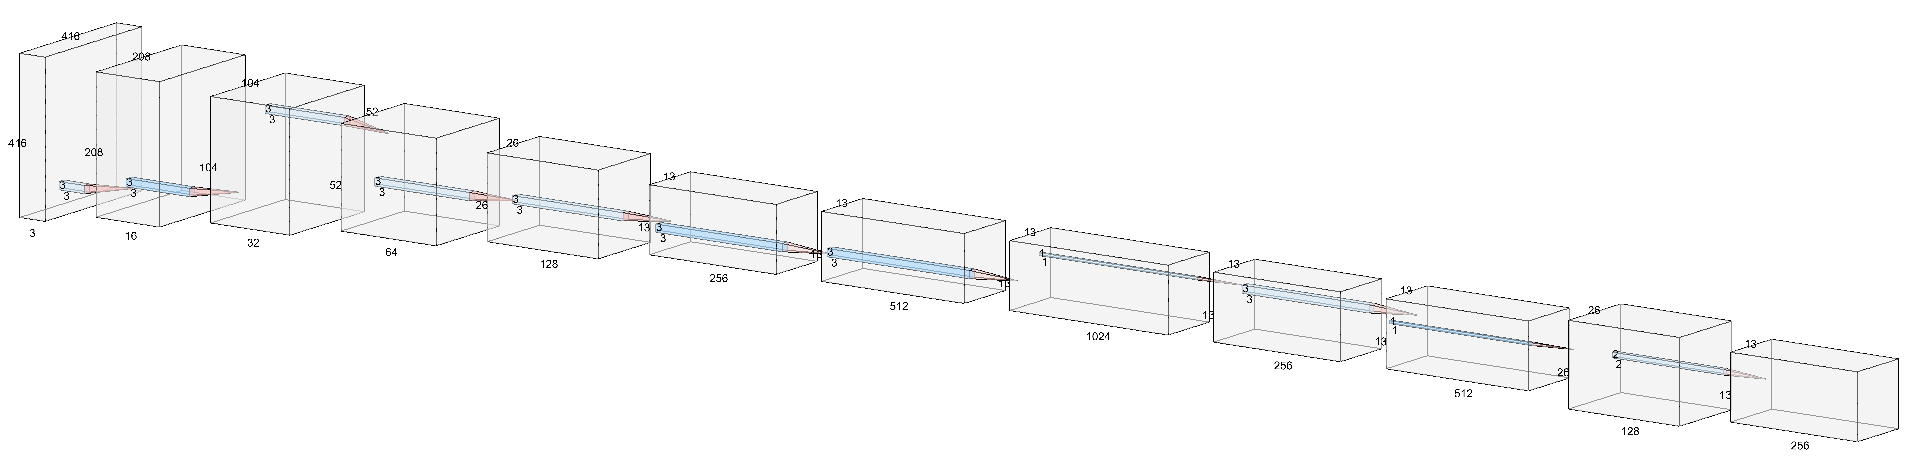
\includegraphics[width=\textwidth]{tinyflat.PNG}
  \caption{YOLOv3 Tiny Architecture Visualized}
  \label{fig:tinyflat}
\end{figure*}

\begin{figure}[h]
  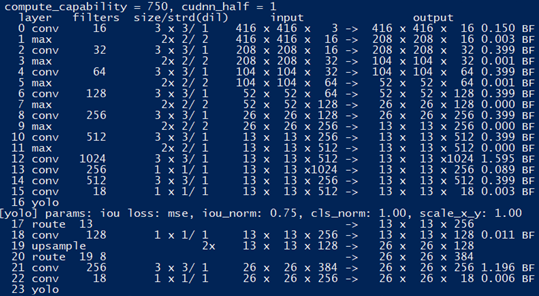
\includegraphics[width=0.45\textwidth]{compute.PNG}
  \caption{The Trained Network}
  \label{fig:compute}
\end{figure}

As should be expected, the most computationally expensive layer to train was the deepest convolutional layer, accounting for more than a quarter of all computation in training. In the second part of the network, where pyramiding occurs, the computation at the second level of scaling suggests either that the dataset may have had poor representation of very large objects, or that this size object was not relevent to the problem. Given that the dataset contained images taken within the full range of zoom allowed in the game, the summary here alone would suggest that for this particular application, a leaner network could shed the large pyramid slice and thus save more training and inference time.

Prior to training I had segmented my original set of images to include 42 randomly-selected testing images against which model performance was assessed in training. 

At a threshold of IoU = 0.5 for ignoring prior boxes and a confidence threshold of 25\%, mAP was 97.3524\%. The table in \textbf{figure 10} below shows more complete performance metrics for a 25\% threshold.

\begin{figure}
    \centering
    \begin{center}
\begin{tabular}{ |c|c| } 
 \hline
 True Positives & 122 \\ 
 False Positives & 2 \\ 
 Precision & 0.98 \\ 
 Recall & 0.98 \\ 
 F1-Score & 0.98 \\ 
 Average IoU & 82.49\% \\ 
 \hline
\end{tabular}
\end{center}
    \caption{Model Performance}
    \label{fig:perf}
\end{figure}

While the accuracy of the model was necessary to its usefulness, equally crucial to its feasibility as a bot-input tool is the speed of its inference. Particularly in the context of an ore-mining bot in Old School Runescape, the network must be able to detect spawned ore quickly enough to signal the bot to begin mining the ore to be competitive with other humans in the pit responding and mining. It was therefore significant that the inference time using OpenCV on CPU was less than 20ms, meaning the bot could be updated more than 50 times a second. 

\subsection{Bot}

The bot consisted of a thin Python wrapper around the CV. In the time constraint I had, there was no time to develop a method of computing box persistence quickly. Therefore I have no way of knowing in frame 2 whether any of the boxes in frame 1 are present in frame 2. This means that after the frame in which I decide to mine an ore, I am not sure when that ore is finished mining. This is significant because in runescape the time to mine is a random roll partially determined by some level inputs, and the bot will almost always be operating in a competitive environment where other players are attempting to mine the same ore when it spawns.

I was forced therefore to simply introduce a random delay between ore retargeting, which I achieve via a stretching of Chi-square on the X axis, where the Y is the probablility of a delay being chosen, and X is that delay. This leads to some efficiency loss, with the bot mining 60-65\% as much as a human in the same pit during an hour of runtime.

While less than ideal, this may actually provide benefit in obfuscation, more efficient bots or players are more likely to be scrutinized by the game developer, where my relatively "slow" bot may not.

\begin{figure}[h]
  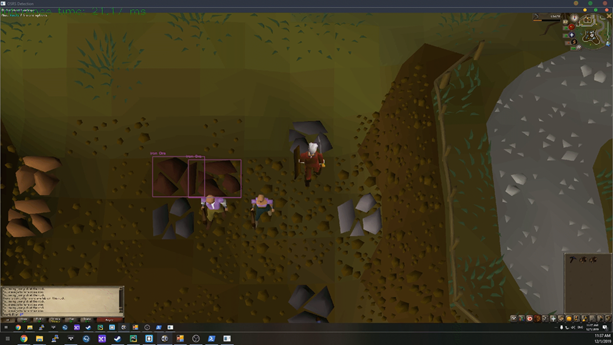
\includegraphics[width=0.45\textwidth]{botaction.PNG}
  \caption{The Bot Monitoring Window}
  \label{fig:botaction}
\end{figure}

\section{Discussion}
\subsection{Broader Bot Feasibility}
In order to be economically feasible, botting has traditionally been carried out at scale with bot farms.\cite{botting} These are swarms of bots that are run in independent VMs or other client sandboxes, connecting across various proxies to imitate player behavior. An IEEE paper exploring the question of botting in games developed a bot-swarm strategy whereby the limits and structure of a game can be determined by random walks through the game with swarms of "ant bots." \cite{Ant} This and bot-farming itself is possible only because of the computational simplicity of such bots, meaning hundreds could be run from a single x86\_64 platform. In the computer vision model, an entire GPU must be devoted to running detection hundreds of times a second with YOLOv3 tiny, or an entire CPU core pegged to capacity with AVX instructions. \cite{YOLO}

Thus while in this paper I have demonstrated that operating a single bot is feasible (at least in games with auto-pathing) using computer vision as the sole means of information input, the applicability of this technique to the broader botting population is extremely limited. My current electricity rate (in one of the cheapest markets in the country) is \$0.104/kWh. Thus the most training the model could have cost me in 18 hours of GPU time, assuming a board-limited peak of 300W, is $.3*18*.104=0.5616$ (ignoring all non-GPU power consumption). While the system load for my desktop of operating the bot was low compared to its total capability, power draw of roughly 350W with the GPU idling during bot execution is still a per-hour cost for \textit{single} bot operation of $.35*0.104=0.0364$. Given an iron-ore farm rate of about 260 per hour with my bot, current (October 9) Grand Exchange Price of iron ore at 52 gold, and RSGilded price for botted gold of \$0.18/million, this method of botting in OSRS would achieve a net hourly loss of $\frac{260*53}{1000000}*0.18-0.0364=-0.0339196$. When you consider the capital outlays necessary for the equipment here used in the RTX 2080, Ryzen 9 3900x, 32GB of binned 3600mhz Micron E-die memory, an X570 chipset and motherboard, a liter reservoir, nickel tube fittings, a d5 pump, copper radiators, etc., it is clear that industrial-scale botting is a long way off absent significant pressure on traditional botting tactics.

\subsection{Anti-Botting}
Conceptually, this new method of providing bot inputs has necessarily fewer detection surfaces than traditional botting. It has all of the detection risks present in normal bots minus any associated with memory access and process injection, making it inherently \textit{less} detectable. 

This is not however to say that this method is a catch-all solution to the issue of anti-bot detection.

I made a naive attempt to determine a patterned difference between bot and human gameplay with 2 hours of recorded mouse and keyboard input during gameplay from my bot and from myself, segmenting the data into equal chunks, extracting actions per second, the average speed of the mouse, the average positional variance, and the average time gap between key-press and mouse-input as inputs to a K-means model and misclassified exactly half of my segmented test periods. My bot did include some random mouse movements, and a randomness around the center of a target click to avoid detection, which was apparently sufficient to defeat simple attempts at categorization.

Jagex however seems to be employing more advanced tools, as my bot was banned 8 days after entering service. It is possible that my bot simply exceeded feasible playtime limits for a human during the period, allowing the developer to surmise that my account was either botting or being shared, both offenses bearing the punishment of a permanent ban, and thus freeing the company from proving which transgression in particular I was committing.

\section{Conclusion}

My goal at the outset of this project was to demonstrate the viability of computer vision as a tool for obtaining game data for any subsequent use. I have done so. While the hardware I used is in no way cheap, neither is it prohibitively expensive. On-par performance could be achieved with a fewer-cored system absent water-cooling and a more cost effective GPU for less than the price of the aluminum-clad potatoes students are so fond of carrying with them.

Although my account was ultimately detected and banned (despite my own simple model's failure to identify a meaningful pattern), my bot made no effort to manipulate heatmaps or camera-angle variation, two sources of data I now know to be in use by Jagex for detection purposes. I am confident that heatmaps could be defeated with greater and more complex randomness in the bot logic, and camera view variation similarly given the robustness of my network to camera-angle changes.

Thus while at the moment the bot may seem impractical and lacking advantage over more traditional alternatives, it is clear that this methodology will eventually become the dominant means of manipulating video games. At its core, the idea of using the direct video output to scrape data exploits a feature so central to games that it cannot be protected; somehow the light must be emitted from the computer to enter the player's eyeball, and if it can enter their eyeball, it can enter a camera lens.

Such a framework is so adaptable that even given perfect hardware controls, bots could be run from smartphones with false mouse input over USB, or Arduinos with cameras attached. Ivan Goncharov has already demonstrated how with an OpenCV for Android port, my YOLOv3 Tiny network could be run \textit{in its present state} from a mobile device on its own camera input.\cite{Android}

I see therefore nothing that can physically prevent the slow encroachment of machine-learning bots into the gaming world where it is profitable. It will be incumbent on game developers then to either create games enjoyable enough that people would rather play them than pay machines to get them to enjoyable parts of the game, design markets and their own offerings such that there is no economic incentive to bot, or promote ever-more-robust adversarial machine learning tools to discern between machines and people on the other side.

\section{Contributions}

I alone contributed to this paper (save the references), as I was unfamiliar with my classmates in the course and came late to the party as it were.



%%
%% The next two lines define the bibliography style to be used, and
%% the bibliography file.
\bibliographystyle{ACM-Reference-Format}
\bibliography{sample-base}

%%
%% If your work has an appendix, this is the place to put it.
\appendix

\section{Work Notes}

I am an economist by training, and am employed by the Federal Reserve in such capacity. I am by no means an engineer and the nature of this work is outside my field of expertise, marginally relevant extreme overclocking, sysadmin, and server experience notwithstanding. I would like to take this opportunity to apologize to the professors and TAs in DSCI 303 for my performance in the course and thank the above for an extremely information-rich semester.
\end{document}
\endinput
%%
%% End of file `sample-sigconf.tex'.
